\section{Isolation (Method): Protocol and Planted Shortcuts}
\label{sec:setting}

\paragraph{Readout and counterfactual images (protocol figure: Supp.~Z).}
We read the log-probabilities of the option letters at the answer position, take the arg\,max as the prediction and the margin (top-1 minus top-2 probability) as the confidence.
Each question is run with the true image and with counterfactuals: a black image, the image of another question, and the nearest-neighbour image (PubMedCLIP~\cite{eslami2023pubmedclip}), a plausible wrong one.
\emph{Text saturation} is the margin $m_b$ with the black image; with $\tau$ the 15th percentile of the margins of 700 unlabeled validation questions, a question is \HI{} (text-decisive) if $m_b\ge\tau$, \LO{} (text-undecided) if $m_b<0.90$ and \MID{} otherwise.
The \emph{image benefit} is $g=\mathrm{acc}(\text{image})-\mathrm{acc}(\text{black image})$ (points); an \emph{override} is a prediction that differs from the black-image answer.
The \emph{blind ceiling} of a benchmark is the accuracy of an option-level classifier that sees neither the question nor the image, and its \emph{visual headroom} is the true-image accuracy of a fine-tuned model minus the larger of its black-image accuracy and the blind ceiling (Supp.~Z).

\paragraph{Visual ladder and planted shortcuts.}
To vary the visual evidence we replace the true image by Gaussian blurs of radius 32, 16, 8, 4 and 2\,px (on the 448\,px image) and by the intact image.
To vary the shortcut we plant a neutral nonvisual cue at a controlled strength $d$, the share of questions in which the correct option carries it: neutral filler words on all options so that the correct option is the shortest (\emph{length}), or the correct option placed at position A (\emph{position}); training and test options are planted alike, the realised rate equals $d$ to within one question, and $d=0.25$ is a control that carries the same filler without a cue.

\paragraph{Benchmarks and systems.}
\emph{Med-CMR}: 14{,}398 five-option training MCQs, a frozen 711-question test slice and a pool of 16{,}836 further cases for fresh samples (case-disjoint and near-duplicate-filtered; no patient identifiers exist).
\emph{PMC-VQA}~\cite{zhang2023pmcvqa}: four-option questions on PubMed Central figures (9{,}277 training, 1{,}999 clean test, 3{,}000 held-out).
\emph{OmniMedVQA}~\cite{hu2024omnimedvqa} (open-access subset) and \emph{A-OKVQA}~\cite{schwenk2022aokvqa} (photographs; the 1{,}145 validation questions are the test set).
Systems: the released adapter of a top-3 MedReason~2026 system (Qwen3.5-9B, 4-bit, rank-16 LoRA~\cite{hu2022lora}; test accuracy 683/711 reproduced) and public models fine-tuned by us with one recipe: Qwen2.5-VL-3B and -7B~\cite{bai2025qwen25vl} and InternVL3-2B~\cite{zhu2025internvl3} (LoRA $r{=}16$ on the language layers, one epoch, learning rate $10^{-4}$, images at most 448\,px, loss on the answer letter).
All experiments follow one pre-specification with dated amendments, each frozen and SHA-256-hashed before the run it governs (the hashes are self-held, not an external registry); criteria fixed after earlier results are marked where they occur, and failed and not-evaluable tests are reported.

\begin{figure*}[t]
  \centering
  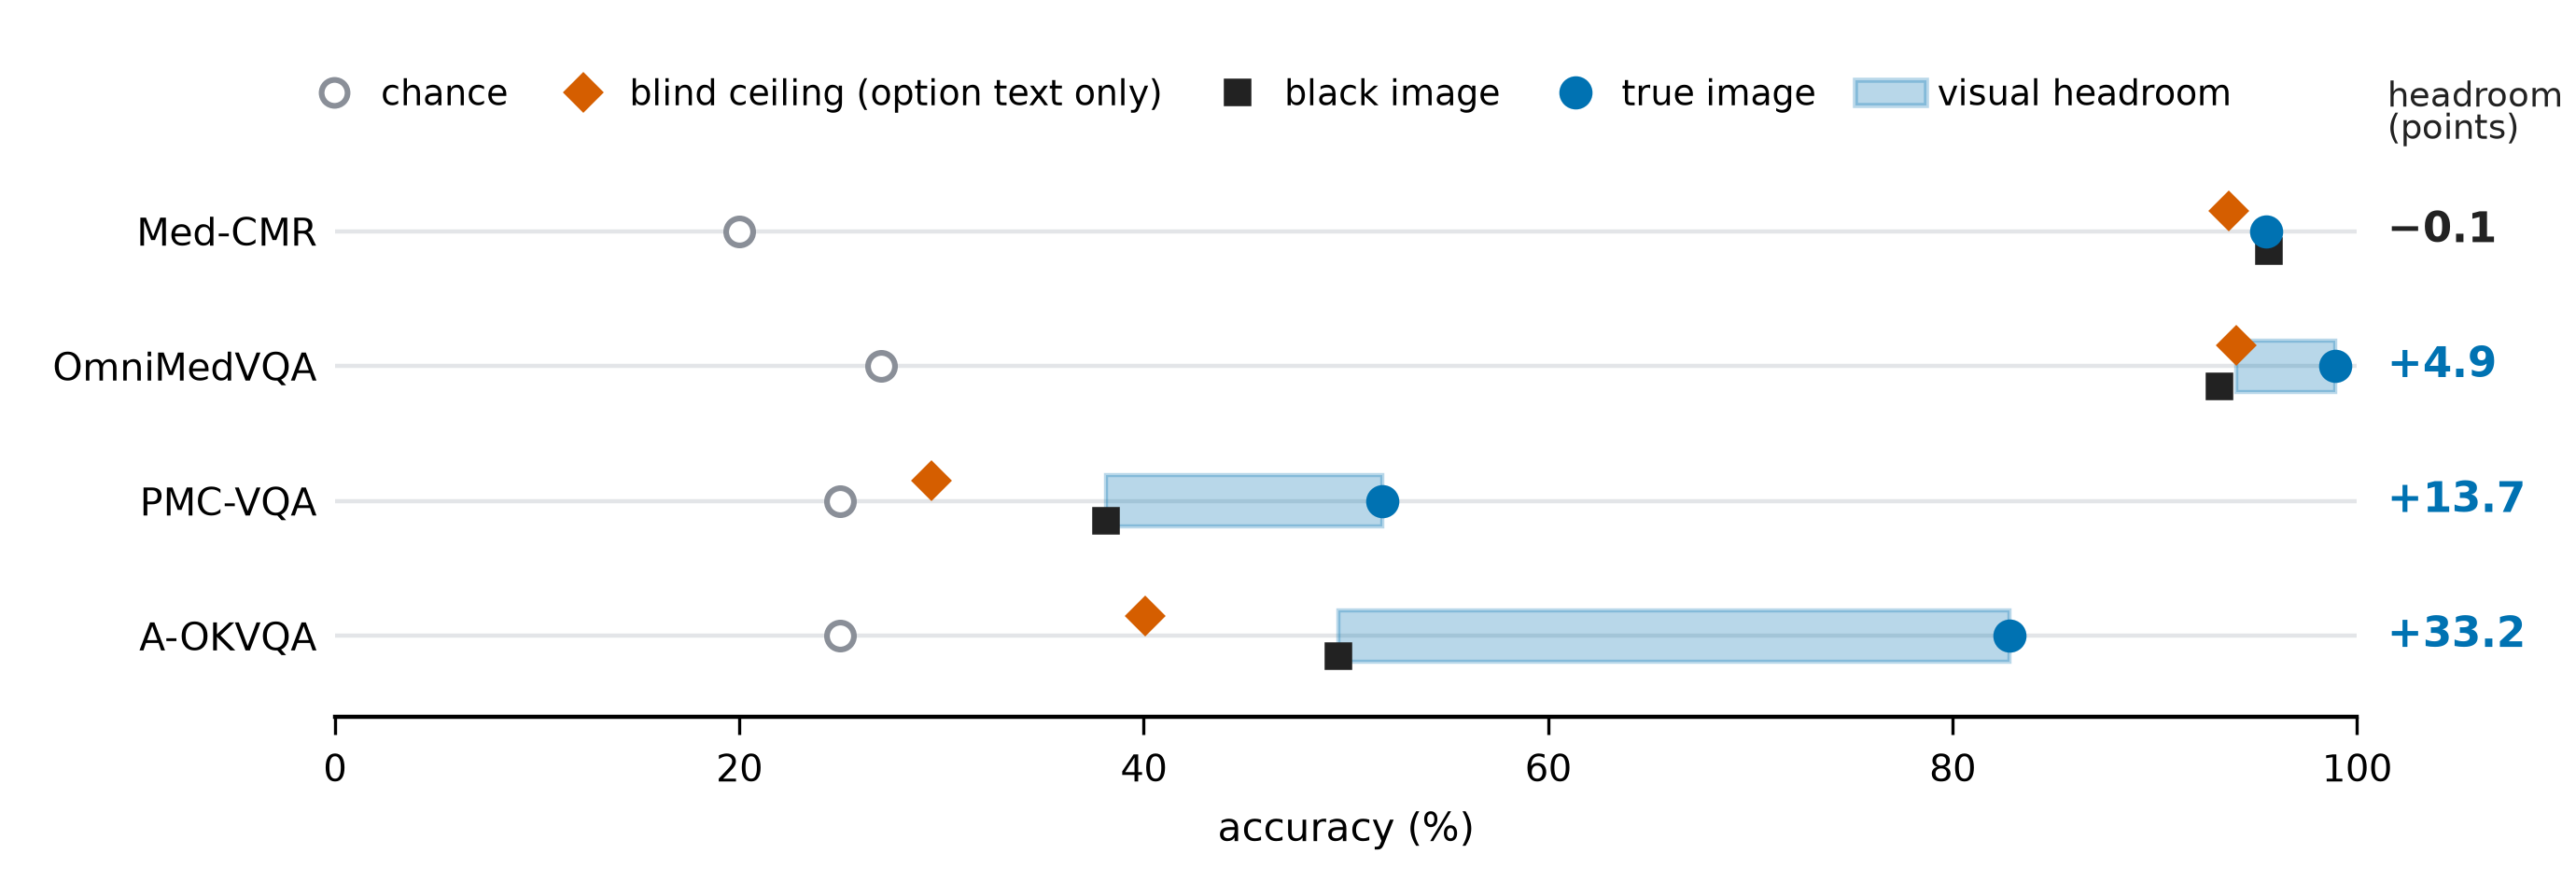
\includegraphics[width=0.74\textwidth]{fig/f2_headroom.png}
  \caption{\textbf{Visual headroom of four benchmarks} (fine-tuned Qwen2.5-VL-3B, held-out questions). Chance, the blind ceiling (an option-level classifier that sees neither the question nor the image), and the accuracy with a black image and with the true image; the shaded interval is the true-image accuracy above both no-image marks, i.e.\ the visual headroom (points, right).}
  \label{fig:headroom}
\end{figure*}

\paragraph{A contrast, observational.}
Headroom differs widely (Fig.~\ref{fig:headroom}): $-0.1$ points on Med-CMR (blind ceiling $93.7\%$), $+4.9$ on OmniMedVQA ($94.1\%$, with no length cue; we did not test why its blind ceiling is high), $+13.7$ on PMC-VQA ($29.5\%$) and $+33.2$ on A-OKVQA ($40.1\%$; fine-tuned Qwen-3B, Supp.~Z).
On PMC-VQA the correct option is the shortest in only 19.7\% of the questions; the same three families with the identical recipe do not acquire the habit (24--27\%), are never text-decisive (no black-image margin of at least $0.99$, against 75--79\% on Med-CMR) and lose $13.7$, $14.9$ and $14.4$ points without the image (Supp.~Z).
The benchmarks differ in topic and style, so this contrast is observational; planting the shortcut is the controlled test (Sec.~\ref{sec:dose}).
